\subsection{Basiswahl
\label{buch:subsection:basiswahl}}
Die Definition der Homologiegruppen $H_k(C)$ als Quotient von
Vektorräumen ist ziemlich abstrakt.
Sie besteht aus Klassen von Zyklen, die sich höchstens um einen
Rand unterscheiden.
Indem wir eine geeignete Basis wählen, können wir konkrete Zyklen
identifizieren, die eine Basis für den Vektorraum $H_k(C)$ bilden.
Dies soll im Folgenden schrittweise durchgeführt werden.

\begin{figure}
\centering
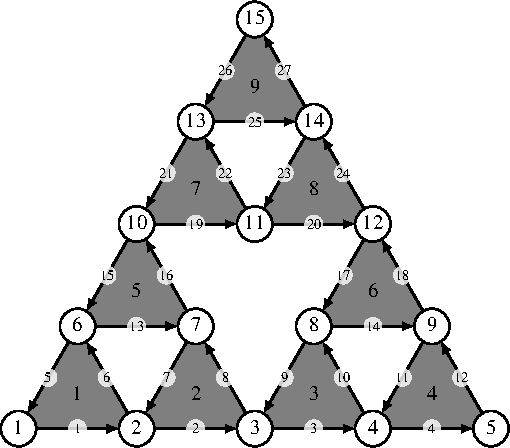
\includegraphics{chapters/95-homologie/images/gausshomoex.pdf}
\caption{Beispiel für die Berechnung von Basisvektoren und Homologieklassen
mit Hilfe des Gauss-Algorithmus
\label{buch:homologie:fig:gausshomoex}}
\end{figure}

\subsubsection{Basis von $Z_k(C)$}
Um eine Basis für $H_k(C)$ zu konstruieren, ist es zunächst nötig,
eine Basis der Zyklen $Z_k(C)$ zu bestimmen.
Ausgehend von einer beliebigen Basis der $C_k$ und einer 
zugehörigen Darstellung des Randoperators $\partial_k$ als
Matrix, kann eine Basis von Zyklen mit Hilfe des Gauss-Algorithmus
gefunden werden.
Wir bezeichnen die Menge dieser Zyklen mit
\[
\mathcal{Z}_k 
=
\{
z_1^{(k)},
z_2^{(k)},
\dots,
z_l^{(k)}
\}.
\]
$\mathcal{Z}_k$ erzeugt den $l$-dimensionalen Vektorraum $Z_k(C)$.

\begin{beispiel}
\label{buch:homologie:beispiel:gausshomo}
In Abbildung~\ref{buch:homologie:fig:gausshomoex} ist ein Polyeder 
dargestellt, dessen Homologiegruppe $H_1$ berechnet werden soll.
Um eine Basis für die Zyklen zu berechnen, wird zunächst die Matrix
des Randoperators $\partial_1$ aufgestellt.
Sie ist
\[
\setcounter{MaxMatrixCols}{27}
\partial_1
=
\footnotesize
\setlength\arraycolsep{2pt}
\begin{pmatrix*}[r]
%1  2  3  4  5  6  7  8  9 10 11 12 13 14 15 16 17 18 19 20 21 22 23 24 25 26 27
-1& 0& 0& 0&-1& 0& 0& 0& 0& 0& 0& 0& 0& 0& 0& 0& 0& 0& 0& 0& 0& 0& 0& 0& 0& 0& 0\\ % 1
 1&-1& 0& 0& 0&-1& 1& 0& 0& 0& 0& 0& 0& 0& 0& 0& 0& 0& 0& 0& 0& 0& 0& 0& 0& 0& 0\\ % 2
 0& 1&-1& 0& 0& 0& 0&-1& 1& 0& 0& 0& 0& 0& 0& 0& 0& 0& 0& 0& 0& 0& 0& 0& 0& 0& 0\\ % 3
 0& 0& 1&-1& 0& 0& 0& 0& 0&-1& 1& 0& 0& 0& 0& 0& 0& 0& 0& 0& 0& 0& 0& 0& 0& 0& 0\\ % 4
 0& 0& 0& 1& 0& 0& 0& 0& 0& 0& 0&-1& 0& 0& 0& 0& 0& 0& 0& 0& 0& 0& 0& 0& 0& 0& 0\\ % 5
 0& 0& 0& 0& 1& 1& 0& 0& 0& 0& 0& 0&-1& 0& 1& 0& 0& 0& 0& 0& 0& 0& 0& 0& 0& 0& 0\\ % 6
 0& 0& 0& 0& 0& 0&-1& 1& 0& 0& 0& 0& 1& 0& 0&-1& 0& 0& 0& 0& 0& 0& 0& 0& 0& 0& 0\\ % 7
 0& 0& 0& 0& 0& 0& 0& 0&-1& 1& 0& 0& 0&-1& 0& 0& 1& 0& 0& 0& 0& 0& 0& 0& 0& 0& 0\\ % 8
 0& 0& 0& 0& 0& 0& 0& 0& 0& 0&-1& 1& 0& 1& 0& 0& 0&-1& 0& 0& 0& 0& 0& 0& 0& 0& 0\\ % 9
 0& 0& 0& 0& 0& 0& 0& 0& 0& 0& 0& 0& 0& 0&-1& 1& 0& 0&-1& 0& 1& 0& 0& 0& 0& 0& 0\\ %10
 0& 0& 0& 0& 0& 0& 0& 0& 0& 0& 0& 0& 0& 0& 0& 0& 0& 0& 1&-1& 0&-1& 1& 0& 0& 0& 0\\ %11
 0& 0& 0& 0& 0& 0& 0& 0& 0& 0& 0& 0& 0& 0& 0& 0&-1& 1& 0& 1& 0& 0& 0&-1& 0& 0& 0\\ %12
 0& 0& 0& 0& 0& 0& 0& 0& 0& 0& 0& 0& 0& 0& 0& 0& 0& 0& 0& 0&-1& 1& 0& 0&-1& 1& 0\\ %13
 0& 0& 0& 0& 0& 0& 0& 0& 0& 0& 0& 0& 0& 0& 0& 0& 0& 0& 0& 0& 0& 0&-1& 1& 1& 0&-1\\ %14
 0& 0& 0& 0& 0& 0& 0& 0& 0& 0& 0& 0& 0& 0& 0& 0& 0& 0& 0& 0& 0& 0& 0& 0& 0&-1& 1\\ %15
\end{pmatrix*}
\]
Die reduzierte Zeilenstufenform von $\partial_1$ ist
(Pivotpositionen in {\color{red}rot}, frei wählbare Variablen
in {\color{darkgreen}grün})
\begin{center}
%\tiny
\scriptsize
%\footnotesize
\setlength\tabcolsep{3pt}
\begin{tabular}{|>{$}r<{$}|>{$}r<{$}>{$}r<{$}>{$}r<{$}>{$}r<{$}>{$}r<{$}>{$}r<{$}>{$}r<{$}>{$}r<{$}>{$}r<{$}>{$}r<{$}>{$}r<{$}>{$}r<{$}>{$}r<{$}>{$}r<{$}>{$}r<{$}>{$}r<{$}>{$}r<{$}>{$}r<{$}>{$}r<{$}>{$}r<{$}>{$}r<{$}>{$}r<{$}>{$}r<{$}>{$}r<{$}>{$}r<{$}>{$}r<{$}>{$}r<{$}|}
\hline
  & 1& 2& 3& 4& 5&{\color{darkgreen}6}& 7&{\color{darkgreen}8}& 9&{\color{darkgreen}10}&11&{\color{darkgreen}12}&{\color{darkgreen}13}&{\color{darkgreen}14}&15&{\color{darkgreen}16}&17&{\color{darkgreen}18}&19&{\color{darkgreen}20}&21&{\color{darkgreen}22}&23&{\color{darkgreen}24}&{\color{darkgreen}25}&26&{\color{darkgreen}27}\\
\hline
 1&\phantom{-}{\color{red}1}& 0& 0& 0& 0&-1& 0& 0& 0& 0& 0& 0& 1& 0& 0&-1& 0& 0& 0& 1& 0& 0& 0&-1& 0& 0& 0\\
 2& 0&\phantom{-}{\color{red}1}& 0& 0& 0& 0& 0&-1& 0& 0& 0& 0& 0& 0& 0& 0& 0& 0& 0& 1& 0& 0& 0&-1& 0& 0& 0\\
 3& 0& 0&\phantom{-}{\color{red}1}& 0& 0& 0& 0& 0& 0&-1& 0& 0& 0& 1& 0& 0& 0&-1& 0& 0& 0& 0& 0& 0& 0& 0& 0\\
 4& 0& 0& 0&\phantom{-}{\color{red}1}& 0& 0& 0& 0& 0& 0& 0&-1& 0& 0& 0& 0& 0& 0& 0& 0& 0& 0& 0& 0& 0& 0& 0\\
 5& 0& 0& 0& 0&\phantom{-}{\color{red}1}&-1& 0& 0& 0& 0& 0& 0& 1& 0& 0&-1& 0& 0& 0& 1& 0& 0& 0&-1& 0& 0& 0\\
 6& 0& 0& 0& 0& 0& 0&\phantom{-}{\color{red}1}&-1& 0& 0& 0& 0&-1& 0& 0& 1& 0& 0& 0& 0& 0& 0& 0& 0& 0& 0& 0\\
 7& 0& 0& 0& 0& 0& 0& 0& 0&\phantom{-}{\color{red}1}&-1& 0& 0& 0& 1& 0& 0& 0&-1& 0&-1& 0& 0& 0& 1& 0& 0& 0\\
 8& 0& 0& 0& 0& 0& 0& 0& 0& 0& 0&\phantom{-}{\color{red}1}&-1& 0&-1& 0& 0& 0& 1& 0& 0& 0& 0& 0& 0& 0& 0& 0\\
 9& 0& 0& 0& 0& 0& 0& 0& 0& 0& 0& 0& 0& 0& 0&\phantom{-}{\color{red}1}&-1& 0& 0& 0& 1& 0& 0& 0&-1& 0& 0& 0\\
10& 0& 0& 0& 0& 0& 0& 0& 0& 0& 0& 0& 0& 0& 0& 0& 0&\phantom{-}{\color{red}1}&-1& 0&-1& 0& 0& 0& 1& 0& 0& 0\\
11& 0& 0& 0& 0& 0& 0& 0& 0& 0& 0& 0& 0& 0& 0& 0& 0& 0& 0&\phantom{-}{\color{red}1}&-1& 0&-1& 0& 1& 1& 0&-1\\
12& 0& 0& 0& 0& 0& 0& 0& 0& 0& 0& 0& 0& 0& 0& 0& 0& 0& 0& 0& 0&\phantom{-}{\color{red}1}&-1& 0& 0& 1& 0&-1\\
13& 0& 0& 0& 0& 0& 0& 0& 0& 0& 0& 0& 0& 0& 0& 0& 0& 0& 0& 0& 0& 0& 0&\phantom{-}{\color{red}1}&-1&-1& 0& 1\\
14& 0& 0& 0& 0& 0& 0& 0& 0& 0& 0& 0& 0& 0& 0& 0& 0& 0& 0& 0& 0& 0& 0& 0& 0& 0&\phantom{-}{\color{red}1}&-1\\
15& 0& 0& 0& 0& 0& 0& 0& 0& 0& 0& 0& 0& 0& 0& 0& 0& 0& 0& 0& 0& 0& 0& 0& 0& 0& 0& 0\\
\hline
\end{tabular}.
\end{center}
Daraus kann man die Zyklen wie folgt ablesen, indem man jeweils
genau eine frei wählbare Variable auf $1$ setzt:
\begin{align*}
z_1
&=
\tiny
\begin{pmatrix*}[r]
\phantom{-}
 1\\
 0\\
 0\\
 0\\
 1\\
 1\\
 0\\
 0\\
 0\\
 0\\
 0\\
 0\\
 0\\
 0\\
 0\\
 0\\
 0\\
 0\\
 0\\
 0\\
 0\\
 0\\
 0\\
 0\\
 0\\
 0\\
 0
\end{pmatrix*},
&
\phantom{\mathstrut_0}
z_2
&=
\tiny
\begin{pmatrix*}[r]
\phantom{-}
 0\\
 1\\
 0\\
 0\\
 0\\
 0\\
 1\\
 1\\
 0\\
 0\\
 0\\
 0\\
 0\\
 0\\
 0\\
 0\\
 0\\
 0\\
 0\\
 0\\
 0\\
 0\\
 0\\
 0\\
 0\\
 0\\
 0
\end{pmatrix*},
&z_3
&=
\tiny
\begin{pmatrix*}[r]
\phantom{-}
 0\\
 0\\
 1\\
 0\\
 0\\
 0\\
 0\\
 0\\
 1\\
 1\\
 0\\
 0\\
 0\\
 0\\
 0\\
 0\\
 0\\
 0\\
 0\\
 0\\
 0\\
 0\\
 0\\
 0\\
 0\\
 0\\
 0
\end{pmatrix*},
&z_4 % variable 12 = 1
&=
\tiny
\begin{pmatrix*}[r]
\phantom{-}
 0\\
 0\\
 0\\
 1\\
 0\\
 0\\
 0\\
 0\\
 0\\
 0\\
 1\\
 1\\
 0\\
 0\\
 0\\
 0\\
 0\\
 0\\
 0\\
 0\\
 0\\
 0\\
 0\\
 0\\
 0\\
 0\\
 0
\end{pmatrix*},
&z_5 % variable 13 = 1
&=
\tiny
\begin{pmatrix*}[r]
-1\\
 0\\
 0\\
 0\\
-1\\
 0\\
 1\\
 0\\
 0\\
 0\\
 0\\
 0\\
 1\\
 0\\
 0\\
 0\\
 0\\
 0\\
 0\\
 0\\
 0\\
 0\\
 0\\
 0\\
 0\\
 0\\
 0
\end{pmatrix*},
&z_6 % variable 14 = 1
&=
\tiny
\begin{pmatrix*}[r]
 0\\
 0\\
-1\\
 0\\
 0\\
 0\\
 0\\
 0\\
-1\\
 0\\
 1\\
 0\\
 0\\
 1\\
 0\\
 0\\
 0\\
 0\\
 0\\
 0\\
 0\\
 0\\
 0\\
 0\\
 0\\
 0\\
 0
\end{pmatrix*},
&z_7 % variable 16 = 1
&=
\tiny
\begin{pmatrix*}[r]
 1\\
 0\\
 0\\
 0\\
 1\\
 0\\
-1\\
 0\\
 0\\
 0\\
 0\\
 0\\
 0\\
 0\\
 1\\
 1\\
 0\\
 0\\
 0\\
 0\\
 0\\
 0\\
 0\\
 0\\
 0\\
 0\\
 0
\end{pmatrix*},\\
z_8 % variable 18 = 1
&=
\tiny
\begin{pmatrix*}[r]
 0\\
 0\\
 1\\
 0\\
 0\\
 0\\
 0\\
 0\\
 1\\
 0\\
-1\\
 0\\
 0\\
 0\\
 0\\
 0\\
 1\\
 1\\
 0\\
 0\\
 0\\
 0\\
 0\\
 0\\
 0\\
 0\\
 0
\end{pmatrix*},
&z_9 % variable 20 = 1
&=
\tiny
\begin{pmatrix*}[r]
-1\\
-1\\
 0\\
 0\\
-1\\
 0\\
 0\\
 0\\
 1\\
 0\\
 0\\
 0\\
 0\\
 0\\
-1\\
 0\\
 1\\
 0\\
 1\\
 1\\
 0\\
 0\\
 0\\
 0\\
 0\\
 0\\
 0
\end{pmatrix*},
&z_{10} % variable 22 = 1
&=
\tiny
\begin{pmatrix*}[r]
\phantom{-}
 0\\
 0\\
 0\\
 0\\
 0\\ %5
 0\\ 
 0\\
 0\\
 0\\
 0\\ %10
 0\\ 
 0\\
 0\\
 0\\
 0\\ %15
 0\\
 0\\
 0\\
 1\\
 0\\ %20
 1\\
 1\\
 0\\
 0\\
 0\\ %25
 0\\
 0
\end{pmatrix*},
&z_{11} % variable 24 = 1
&=
\tiny
\begin{pmatrix*}[r]
 1\\
 1\\
 0\\
 0\\
 1\\ %5
 0\\
 0\\
 0\\
-1\\
 0\\ %10
 0\\
 0\\
 0\\
 0\\
 1\\ %15
 0\\
-1\\
 0\\
-1\\
 0\\ %20
 0\\
 0\\
 1\\
 1\\
 0\\ %25
 0\\
 0
\end{pmatrix*},
&z_{12} % variable 25 = 1
&=
\tiny
\begin{pmatrix*}[r]
 0\\
 0\\
 0\\
 0\\
 0\\
 0\\
 0\\
 0\\
 0\\
 0\\ %10
 0\\
 0\\
 0\\
 0\\
 0\\ %15
 0\\
 0\\
 0\\
-1\\
 0\\ %20
-1\\
 0\\
 1\\
 0\\
 1\\ %25
 0\\
 0
\end{pmatrix*},
&z_{13} % variable 27 = 1
&=
\tiny
\begin{pmatrix*}[r]
 0\\
 0\\
 0\\
 0\\
 0\\
 0\\
 0\\
 0\\
 0\\
 0\\
 0\\
 0\\
 0\\
 0\\
 0\\
 0\\
 0\\
 0\\
 1\\
 0\\ %20
 1\\
 0\\
-1\\
 0\\
 0\\ %25
 1\\
 1
\end{pmatrix*}.
\end{align*}
\begin{figure}
\centering
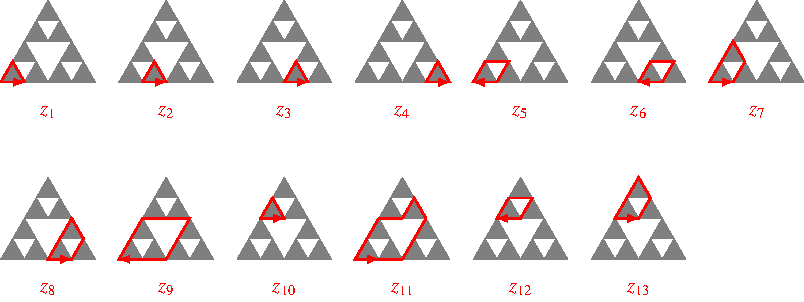
\includegraphics{chapters/95-homologie/images/homocycles.pdf}
\caption{Zyklen des Randoperators $\partial_1$ im Beispiel von
Seite~\pageref{buch:homologie:beispiel:gausshomo}.
\label{buch:homologie:fig:homocycles}}
\end{figure}%
Die Zyklen sind in Abbildung~\ref{buch:homologie:fig:homocycles} {\color{red}rot} dargestellt.
\end{beispiel}

\subsubsection{Basis für $B_k(C)$}
Da $B_k(C)\subset Z_k(C)$ gilt, lässt sich für jedes $c_{k+1}\in C_{k+1}$
der Rand $\partial_{k+1}c_{k+1}$ als Linearkombination der im 
vorangegangenen Schritt gefundenen Basiszyklen finden.
Wir können also aus der Standardbasis $e^{(k+1)}_i\in C_{k+1}$ eine Menge
von Vektoren $\partial_{k+1}e^{(k+1)}_i$ gewinnen, die mit Sicherheit
ganz $B_k(C)$ aufspannen.
Es ist aber davon auszugehen, dass diese Vektoren nicht linear unabhängig
sind.
Es ist also nötig, eine Teilmenge
\[
\mathcal{B}_k
=
\{
\partial_{k+1}e^{(k+1)}_{i_1},
\partial_{k+1}e^{(k+1)}_{i_2},
\dots,
\partial_{k+1}e^{(k+1)}_{i_m}
\}
\]
von Vektoren auszuwählen, die linear
unabhängig sind.
Diese bilden eine Basis von $B_k(C)$ und sind als
blaue Dreiecke in Abbildung~\ref{buch:homologie:fig:homoboundaries}
dargestellt.

\begin{figure}
\centering
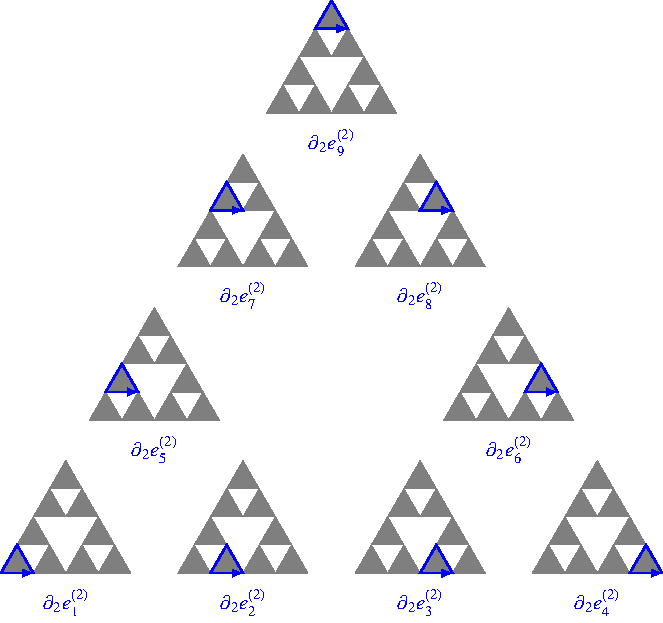
\includegraphics{chapters/95-homologie/images/homoboundaries.pdf}
\caption{Die Ränder $\partial_2e_i^{(2)}$ für das Beispiel von
Seite~\pageref{buch:homologie:beispiel:gausshomo}.
Die grauen Dreiecke bilden die Standardbasis $e_i^{(2)}$ von $C_2$,
die blauen Dreiecke sind die Ränder $\partial_2e_i^{(2)}$ dieser
Dreiecke.
\label{buch:homologie:fig:homoboundaries}}
\end{figure}

Aus den Abbildungen~\ref{buch:homologie:fig:homocycles} und
\ref{buch:homologie:fig:homoboundaries} kann man auch ablesen,
wie die Ränder $\partial_2e_i^{(2)}$ aus den Zyklen von $\mathcal{Z}_1$
linear kombiniert werden können.
Man erhält so die Beziehungen
\begin{equation}
\setcounter{MaxMatrixCols}{29}
\setlength\arraycolsep{1pt}
\begin{array}{lcrcrcrcrcrcrcrcrcrcrcrcrcr}
\partial_2e_1^{(2)} &=&z_1& &   & &   & &   & &   & &   & &   & &   & &   & &      & &      & &      & &      \\
\partial_2e_2^{(2)} &=&   & &z_2& &   & &   & &   & &   & &   & &   & &   & &      & &      & &      & &      \\
\partial_2e_3^{(2)} &=&   & &   & &z_3& &   & &   & &   & &   & &   & &   & &      & &      & &      & &      \\
\partial_2e_4^{(2)} &=&   & &   & &   & &z_4& &   & &   & &   & &   & &   & &      & &      & &      & &      \\
\partial_2e_5^{(2)} &=&   & &   & &   & &   & &z_5& &   &+&z_7& &   & &   & &      & &      & &      & &      \\
\partial_2e_6^{(2)} &=&   & &   & &   & &   & &   & &z_6& &   &+&z_8& &   & &      & &      & &      & &      \\
\partial_2e_7^{(2)} &=&   & &   & &   & &   & &   & &   & &   & &   & &   & &z_{10}& &      & &      & &      \\
\partial_2e_8^{(2)} &=&   & &   & &   & &   & &   & &   & &   & &   & &   & &      & &z_{11}& &      & &      \\
\partial_2e_9^{(2)} &=&   &\phantom{+}&   &\phantom{+} &   &\phantom{+} &   &\phantom{+} &   &\phantom{+} &   &\phantom{+} &   &\phantom{+} &   &\phantom{+} &   &\phantom{+} &      &\phantom{+} &      & &z_{12}&+&z_{13}.
\end{array}
\end{equation}
Dies reicht jedoch nicht, um herauszufinden, welche der blauen Dreiecke
linear unabhängig sind.
Im vorliegenden Fall ist dies einfach: jedes blaue Dreieck besteht aus
Kanten, die in keinem anderen blauen Dreieck vorkommen, daher müssen
sie alle linear unabhängig sein.

\begin{figure}
\centering
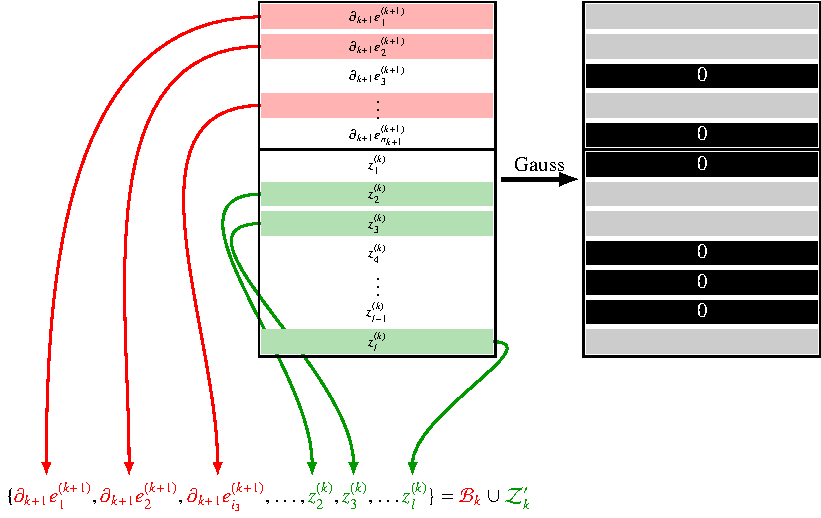
\includegraphics{chapters/95-homologie/images/gausshomobasis.pdf}
\caption{Bestimmung einer Basis für die Homologiegruppe $H_k(C)$ mit
Hilfe der Vorwärtsreduktion des Gaussalgorithmus.
Die schwarzen Nullzeilen zeigen an, welche Zeilenvektoren zusammen mit
den darüberliegenden Vektoren nicht linear unabhängig sind und damit nicht
in Frage kommen für die besuchte Basis.
Übrig bleiben die {\color{red}rot} und {\color{darkgreen}grün} hervorgehobenen
Vektoren.
\label{buch:homologie:fig:gausshomobasis}}
\end{figure}

Diese Auswahl lässt sich sehr leicht mit Hilfe der folgenden
Variante des Gauss-Algorithmus realisieren.
Dazu werden die $n_{k+1}$ Zeilen eines Gauss-Tableaus zunächst mit den Vektoren
$\partial_{k+1}{e_i^{(k+1)}}^t$ gefüllt.
Führt man in diesem Tableau die Vorwärtsreduktion durch, wobei man
entstehende Nullzeilen einfach überspringt, bleiben nur noch Zeilen
übrig, die linear unabhängig sind.
Diese Zeilen entsprechen den linear unabhängigen Vektoren von $\mathcal{B}_k$,
die Zeilennummern sind $i_1,i_2,\dots,i_m$.
Dieses Vorgehen ist schematisch im oberen Teil der
Abbildung~\ref{buch:homologie:fig:gausshomobasis} dargestellt.

\subsubsection{Basis für die Homologiegruppe $H_k(C)$}
Um eine Basis von $H_k(C)$ zu konstruieren, müssen wir jetzt eine
Basis von Zyklen finden, die sich nicht nur um einen Rand unterscheiden,
die also zu verschiedenen Homologie-Klassen in $H_k(C)$ gehören.
Gesucht sind jetzt also Vektoren $\mathcal{Z}'_k$ derart, dass 
die Vektoren von $\mathcal{Z}'_k\cup\mathcal{B}_k$ immer noch $Z_k(C)$
aufspannen, aber zusätzlich linear unabhängig sind.

Dazu kann man wie folgt vorgehen.
\begin{enumerate}
\item
Man beginnt mit $\mathcal{D}_0=\emptyset$ und setzt $j=0$.
\item
Dann testet man der Reihe nach alle noch nicht getesteten Vektoren
von $z_i^{(k)}\in\mathcal{Z}_k$ daraufhin, ob sie von den Vektoren
$\mathcal{B}_k\cup \mathcal{D}_j$ linear unabhängig sind.
Wenn ja, bildet man $\mathcal{D}_{j+1} = \mathcal{D}\cup\{z^{(k)}_i\}$ und
setzt $j=1$.
Andernfalls ignoriert man $z^{(k)}_i$.
\item
Schritt 2 wird wiederholt, bis man alle Vektoren von $\mathcal{Z}_k$
getestet hat.
Die gesuchte Basis setzt sich zusammen  aus $\mathcal{B}_k$ und
$\mathcal{D}_l$,
also
$
\mathcal{Z}_k'
=
\mathcal{B}_k
\cup
\mathcal{D}_l.
$
\end{enumerate}

Dieser Algorithmus kann ebenfalls mit der oben angesprochenen Variante
des Gauss-Algorithmus durchgeführt werden.
Dazu werden die Zeilen $n_k+1$ bis $n_k+1+|\mathcal{Z}_k|$ mit den
Vektoren $z_i^t$.
Dann führt man die Vorwärtsreduktion im ganzen Tableau durch, wobei
man wieder die Nullzeilen stehen lässt.
Nullzeilen zeigen wieder Vektoren an, die sich linear durch die darüber
liegenden Vektoren ausdrücken lassen.
Die auszuwählenden Vektoren sind daher genau diejenigen, die für
$\mathcal{Z}_k'$ ausgewählt werden müssen.


\begin{figure}
\centering
\setlength\tabcolsep{1pt}
\begin{tabular}{|>{$}c<{$}|>{$}r<{$}>{$}r<{$}>{$}r<{$}>{$}r<{$}>{$}r<{$}>{$}r<{$}>{$}r<{$}>{$}r<{$}>{$}r<{$}>{$}r<{$}|>{$}r<{$}>{$}r<{$}>{$}r<{$}>{$}r<{$}>{$}r<{$}>{$}r<{$}>{$}r<{$}>{$}r<{$}>{$}r<{$}>{$}r<{$}|>{$}r<{$}>{$}r<{$}>{$}r<{$}>{$}r<{$}>{$}r<{$}>{$}r<{$}>{$}r<{$}|}
\hline
&\scriptstyle 1&\scriptstyle 2&\scriptstyle 3&\scriptstyle 4 &\scriptstyle 5
&\scriptstyle 6 &\scriptstyle 7 &\scriptstyle 8 &\scriptstyle 9 &\scriptstyle 10
&\scriptstyle 11 &\scriptstyle 12 &\scriptstyle 13 &\scriptstyle 14 &\scriptstyle 15
&\scriptstyle 16 &\scriptstyle 17 &\scriptstyle 18 &\scriptstyle 19 &\scriptstyle 20
&\scriptstyle 21 &\scriptstyle 22 &\scriptstyle 23 &\scriptstyle 24 &\scriptstyle 25
&\scriptstyle 26 &\scriptstyle 27
\\
%                                1  2  3  4  5  6  7  8  9  0  1  2  3  4  5  6  7  8  9  0  1  2  3  4  5  6  7
\hline
\scriptstyle\partial_2e_1^{(2)}& 1&  &  &  & 1&\phantom{-}1&  &  &  &  &  &  &  &  &  &  &  &  &  &  &  &  &  &  &  &  &  \\
\scriptstyle\partial_2e_2^{(2)}&  & 1&  &  &  &  & 1&\phantom{-}1&  &  &  &  &  &  &  &  &  &  &  &  &  &  &  &  &  &  &  \\
\scriptstyle\partial_2e_3^{(2)}&  &  & 1&  &  &  &  &  &\phantom{-}1&\phantom{-}1&  &  &  &  &  &  &  &  &  &  &  &  &  &  &  &  &  \\
\scriptstyle\partial_2e_4^{(2)}&  &  &  &\phantom{-}1&  &  &  &  &  &  & 1&\phantom{-}1&  &  &  &  &  &  &  &  &  &  &  &  &  &  &  \\
\scriptstyle\partial_2e_5^{(2)}&  &  &  &  &  &  &  &  &  &  &  &  & 1&  & 1&\phantom{-}1&  &  &  &  &  &  &  &  &  &  &  \\
\scriptstyle\partial_2e_6^{(2)}&  &  &  &  &  &  &  &  &  &  &  &  &  &\phantom{-}1&  &  & 1&\phantom{-}1&  &  &  &  &  &  &  &  &  \\
\scriptstyle\partial_2e_7^{(2)}&  &  &  &  &  &  &  &  &  &  &  &  &  &  &  &  &  &  & 1&  &\phantom{-}1& 1&  &  &  &  &  \\
\scriptstyle\partial_2e_8^{(2)}&  &  &  &  &  &  &  &  &  &  &  &  &  &  &  &  &  &  &  &\phantom{-}1&  &  & 1&\phantom{-}1&  &  &  \\
\scriptstyle\partial_2e_9^{(2)}&  &  &  &  &  &  &  &  &  &  &  &  &  &  &  &  &  &  &  &  &  &  &  &  &\phantom{-}1&\phantom{-}1&\phantom{-}1\\
\hline
%                    1  2  3  4  5  6  7  8  9 10 11 12 13 14 15 16 17 18 19 20 21 22 23 24 25 26 27
\scriptstyle z_{ 1}& 1&  &  &  & 1& 1&  &  &  &  &  &  &  &  &  &  &  &  &  &  &  &  &  &  &  &  &  \\
\scriptstyle z_{ 2}&  & 1&  &  &  &  & 1& 1&  &  &  &  &  &  &  &  &  &  &  &  &  &  &  &  &  &  &  \\
\scriptstyle z_{ 3}&  &  & 1&  &  &  &  &  & 1& 1&  &  &  &  &  &  &  &  &  &  &  &  &  &  &  &  &  \\
\scriptstyle z_{ 4}&  &  &  & 1&  &  &  &  &  &  & 1& 1&  &  &  &  &  &  &  &  &  &  &  &  &  &  &  \\
\scriptstyle z_{ 5}&-1&  &  &  &-1&  & 1&  &  &  &  &  & 1&  &  &  &  &  &  &  &  &  &  &  &  &  &  \\
\scriptstyle z_{ 6}&  &  &-1&  &  &  &  &  &-1&  & 1&  &  & 1&  &  &  &  &  &  &  &  &  &  &  &  &  \\
\scriptstyle z_{ 7}& 1&  &  &  & 1&  &-1&  &  &  &  &  &  &  & 1& 1&  &  &  &  &  &  &  &  &  &  &  \\
\scriptstyle z_{ 8}&  &  & 1&  &  &  &  &  & 1&  &-1&  &  &  &  &  & 1& 1&  &  &  &  &  &  &  &  &  \\
\scriptstyle z_{ 9}&-1&-1&  &  & 1&  &  &  & 1&  &  &  &  &  &-1&  & 1& 1& 1&  &  &  &  &  &  &  &  \\
\scriptstyle z_{10}&  &  &  &  &  &  &  &  &  &  &  &  &  &  &  &  &  & 1&  & 1& 1&  &  &  &  &  &  \\
\scriptstyle z_{11}& 1& 1&  &  & 1&  &  &  &-1&  &  &  &  &  & 1&  &-1&  &-1&  &  &  & 1& 1&  &  &  \\
\scriptstyle z_{12}&  &  &  &  &  &  &  &  &  &  &  &  &  &  &  &  &  &  &-1&  &-1&  & 1&  & 1&  &  \\
\scriptstyle z_{13}&  &  &  &  &  &  &  &  &  &  &  &  &  &  &  &  &  &  & 1&  & 1&  &-1&  &  & 1& 1\\
\hline
\end{tabular}
\caption{Gauss-Tableau für die Bestimmung einer Basis von
$H_1$ für das Beispiel. 
Die ersten neuen Zeilen bestehen aus den Bildern der
Basisvektoren von $C_2$.
Im vorliegenden Fall kann man sofort sehen, dass alle diese
Zeilen linear unabhängig sind.
Die folgenden Zeilen sind die Zyklen in $\mathbb{Z}_2$, sie
sind ebenfalls linear unabhängig.
Mit Hilfe der Vorwärtsreduktion müssen jetzt diejenigen
Zeilen elminiert werden, die bereits aus anderen Zyklen
mit Hilfe von Rändern der Zeilen 1--9 kombiniert werden können.
\label{buch:homologie:beispiel:gausstableau}}
\end{figure}

\begin{figure}
\centering
\setlength\tabcolsep{1pt}
\begin{tabular}{|>{$}c<{$}|>{$}r<{$}>{$}r<{$}>{$}r<{$}>{$}r<{$}>{$}r<{$}>{$}r<{$}>{$}r<{$}>{$}r<{$}>{$}r<{$}>{$}r<{$}|>{$}r<{$}>{$}r<{$}>{$}r<{$}>{$}r<{$}>{$}r<{$}>{$}r<{$}>{$}r<{$}>{$}r<{$}>{$}r<{$}>{$}r<{$}|>{$}r<{$}>{$}r<{$}>{$}r<{$}>{$}r<{$}>{$}r<{$}>{$}r<{$}>{$}r<{$}|}
\hline
&\scriptstyle 1&\scriptstyle 2&\scriptstyle 3&\scriptstyle 4 &\scriptstyle 5
&\scriptstyle 6 &\scriptstyle 7 &\scriptstyle 8 &\scriptstyle 9 &\scriptstyle 10
&\scriptstyle 11 &\scriptstyle 12 &\scriptstyle 13 &\scriptstyle 14 &\scriptstyle 15
&\scriptstyle 16 &\scriptstyle 17 &\scriptstyle 18 &\scriptstyle 19 &\scriptstyle 20
&\scriptstyle 21 &\scriptstyle 22 &\scriptstyle 23 &\scriptstyle 24 &\scriptstyle 25
&\scriptstyle 26 &\scriptstyle 27
\\
%                                1  2  3  4  5  6  7  8  9  0  1  2  3  4  5  6  7  8  9  0  1  2  3  4  5  6  7
\hline
\scriptstyle\partial_2e_1^{(2)}&\phantom{-}1&  &  &  &\phantom{-}1&\phantom{-}1&  &  &  &  &  &  &  &  &  &  &  &  &  &  &  &  &  &  &  &  &  \\
\scriptstyle\partial_2e_2^{(2)}&  &\phantom{-}1&  &  &  &  &\phantom{-}1&\phantom{-}1&  &  &  &  &  &  &  &  &  &  &  &  &  &  &  &  &  &  &  \\
\scriptstyle\partial_2e_3^{(2)}&  &  &\phantom{-}1&  &  &  &  &  &\phantom{-}1&\phantom{-}1&  &  &  &  &  &  &  &  &  &  &  &  &  &  &  &  &  \\
\scriptstyle\partial_2e_4^{(2)}&  &  &  &\phantom{-}1&  &  &  &  &  &  &\phantom{-}1&\phantom{-}1&  &  &  &  &  &  &  &  &  &  &  &  &  &  &  \\
\scriptstyle\partial_2e_5^{(2)}&  &  &  &  &  &  &  &  &  &  &  &  & 1&  & 1&\phantom{-}1&  &  &  &  &  &  &  &  &  &  &  \\
\scriptstyle\partial_2e_6^{(2)}&  &  &  &  &  &  &  &  &  &  &  &  &  &\phantom{-}1&  &  & 1&\phantom{-}1&  &  &  &  &  &  &  &  &  \\
\scriptstyle\partial_2e_7^{(2)}&  &  &  &  &  &  &  &  &  &  &  &  &  &  &  &  &  &  & 1&  &\phantom{-}1& 1&  &  &  &  &  \\
\scriptstyle\partial_2e_8^{(2)}&  &  &  &  &  &  &  &  &  &  &  &  &  &  &  &  &  &  &  &\phantom{-}1&  &  & 1&\phantom{-}1&  &  &  \\
\scriptstyle\partial_2e_9^{(2)}&  &  &  &  &  &  &  &  &  &  &  &  &  &  &  &  &  &  &  &  &  &  &  &  &\phantom{-}1&\phantom{-}1&\phantom{-}1\\
\hline
%                     1  2  3  4  5  6  7  8  9 10 11 12 13 14 15 16 17 18 19 20 21 22 23 24 25 26 27
\scriptstyle z_{ 1}'&  &  &  &  &  &  &  &  &  &  &  &  &  &  &  &  &  &  &  &  &  &  &  &  &  &  &  \\
\scriptstyle z_{ 2}'&  &  &  &  &  &  &  &  &  &  &  &  &  &  &  &  &  &  &  &  &  &  &  &  &  &  &  \\
\scriptstyle z_{ 3}'&  &  &  &  &  &  &  &  &  &  &  &  &  &  &  &  &  &  &  &  &  &  &  &  &  &  &  \\
\scriptstyle z_{ 4}'&  &  &  &  &  &  &  &  &  &  &  &  &  &  &  &  &  &  &  &  &  &  &  &  &  &  &  \\
\scriptstyle z_{ 5}'&  &  &  &  &  & 1& 1&  &  &  &  &  &  &  &-1&-1&  &  &  &  &  &  &  &  &  &  &  \\
\scriptstyle z_{ 6}'&  &  &  &  &  &  &  &  &  & 1& 1&  &  &  &  &  &-1&-1&  &  &  &  &  &  &  &  &  \\
\scriptstyle z_{ 7}'&  &  &  &  &  &  &  &  &  &  &  &  &  &  &  &  &  &  &  &  &  &  &  &  &  &  &  \\
\scriptstyle z_{ 8}'&  &  &  &  &  &  &  &  &  &  &  &  &  &  &  &  &  &  &  &  &  &  &  &  &  &  &  \\
\scriptstyle z_{ 9}'&  &  &  &  &  &  &  & 1& 1&  &  &  &  &  &  & 1& 1&  &  &  &-1&-1&-1&-1&  &  &  \\
\scriptstyle z_{10}'&  &  &  &  &  &  &  &  &  &  &  &  &  &  &  &  &  &  &  &  &  &  &  &  &  &  &  \\
\scriptstyle z_{11}'&  &  &  &  &  &  &  &  &  &  &  &  &  &  &  &  &  &  &  &  &  &  &  &  &  &  &  \\
\scriptstyle z_{12}'&  &  &  &  &  &  &  &  &  &  &  &  &  &  &  &  &  &  &  &  &  & 1& 1&  &  &-1&-1\\
\scriptstyle z_{13}'&  &  &  &  &  &  &  &  &  &  &  &  &  &  &  &  &  &  &  &  &  &  &  &  &  &  &  \\
\hline
\end{tabular}
\caption{Nach Durchführung der Vorwärtsreduktion kann man die Zyklen
ablesen, die nicht für eine Basis von $H_1$ gebraucht werden.
Die resultierenden Zyklen sind in Abbildung~\ref{buch:homologie:beispiel:homoclasses}
dargestellt.
\label{buch:homologie:beispiel:gausstableaureduziert}}
\end{figure}

\begin{figure}
\centering
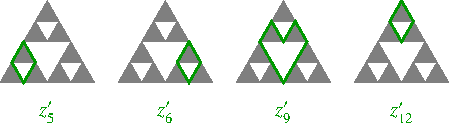
\includegraphics{chapters/95-homologie/images/homoclasses.pdf}
\caption{Repräsentanten für die reduzierten Klassen aus dem
Tableau von
Abbildung~\ref{buch:homologie:beispiel:gausstableaureduziert},
sie bilden eine Basis der Homologie-Gruppe $H_1$.
Jeder dieser Repräsentanten umschliesst genau ein ``Loch'',
also genau ein weisses Dreieck.
\label{buch:homologie:beispiel:homoclasses}}
\end{figure}

\begin{figure}
\centering
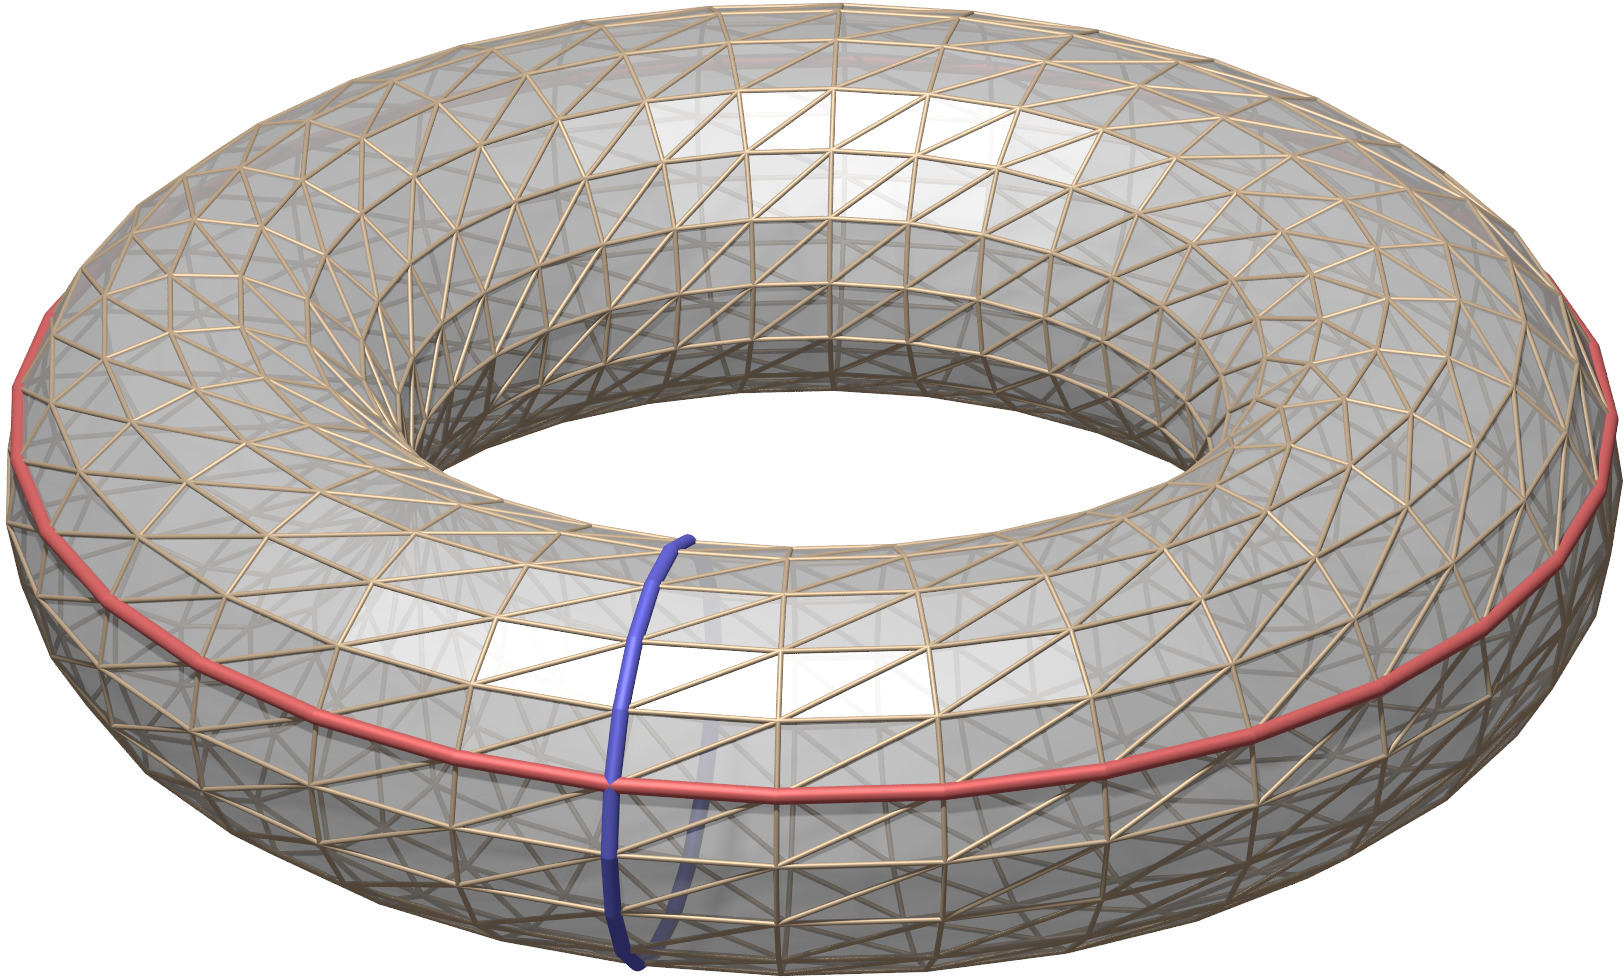
\includegraphics[width=\textwidth]{chapters/95-homologie/torus/torus.jpg}
\caption{Basis der Homologiegruppen eines Torus $T^2$.
Der Algorithmus findet zwei Basisklassen für $H(T^2)$, der eine Zyklus
geht durch das ``Loch'' des Torus (blau), der andere folgt 
dem Äquator.
\label{buch:homologie:fig:torus}}
\end{figure}

Um den Algorithmus für das Beispiel durchzuführen, bilden wir daher das Gauss-Tableau
in Abbildung~\ref{buch:homologie:beispiel:gausstableau},
bestehend aus den Vektoren $\partial_2e_i^{(2)}$ in den ersten 9
Zeilen und den Zyklen $z_1,\dots,z_{13}$ in den folgenden 13 Zeilen.
Das reduzierte Tableau nach der Vorwärtsreduktion ist in
Abbildung~\ref{buch:homologie:beispiel:gausstableaureduziert}
dargestellt, man erkennt, dass die Zyklen $z_1$ bis $z_4$, $z_7$ und $z_8$,
$z_9$ und $z_{10}$ sowie $z_{13}$ weggelassen werden müssen.
Es bleiben die folgenden Zyklen:
\begin{center}
\begin{tabular}{>{$}l<{$}l}
\text{Zyklus}&Eigenschaft\\
\hline
z_5   &Zyklus umschliesst das kleine weisse Dreieck links unten\\
z_6   &Zyklus umschliesst das kleine weisse Dreieck rechts unten\\
z_9   &Zyklus umschliesst das grosse weisse Dreieck\\
z_{12}&Zyklus umschliesst das kleine weisse Dreicke oben\\
\hline
\end{tabular}
\end{center}
Die Zyklen, die nach der Reduktion übrig bleiben, sind in
Abbildung~\ref{buch:homologie:beispiel:homoclasses} zusammengestellt.
Jede solche Klasse entspricht genau einem der ``Löcher'', der weissen
Dreiecke.
Die Homologie kann man also als eine exakte Version der Idee eines
Vektorraums erzeugt von den ``Löchern'' eines Polyeders verstehen.

\subsubsection{Basis von $H_k(C)$}
Die im vorangegangenen Abschnitt konstruierte Basis kann jetzt auch
dazu verwendet werden, eine Basis von $H_k(C)$ zu finden.
Die Vektoren in $\mathcal{B}_k$ bilden eine Basis von $B_k(C)$
und die Vektoren in $\mathcal{Z}_k'$ sind davon unabhängig.
Die Klassen der Vektoren von $\mathcal{Z}_k'$ in $H_k(C)$ sind
daher ebenfalls linear unabhängig und bilden damit eine Basis
von $H_k(C)$.
Die von obigem Algorithmus ausgewählten Zyklen bilden also automatisch
eine Basis von Zyklen, die nicht Rand irgend einer Kette in $C_{k+1}$
sein können.


Führt man das beschriebene Verfahren für einen zweidimensionalen Torus $T^2$ durch,
findet es die beiden in Abbildung~\ref{buch:homologie:fig:torus} dargestellten
Zyklen.
Sie zeigen schön, wie die Homologieklassen die beiden Arten von ``Löchern''
erkennen.
Zum einen ist da der blaue Zyklus, der das ``Loch'' im Inneren des Torus
umschliesst.
Der rote Zyklus dagegen folgt ungefähr dem Äquator und repräsentiert
damit die ``Ringform'' des Torus.
